\documentclass[a4paper]{article}\usepackage[]{graphicx}\usepackage[]{color}
%% maxwidth is the original width if it is less than linewidth
%% otherwise use linewidth (to make sure the graphics do not exceed the margin)
\makeatletter
\def\maxwidth{ %
  \ifdim\Gin@nat@width>\linewidth
    \linewidth
  \else
    \Gin@nat@width
  \fi
}
\makeatother

\definecolor{fgcolor}{rgb}{0.345, 0.345, 0.345}
\newcommand{\hlnum}[1]{\textcolor[rgb]{0.686,0.059,0.569}{#1}}%
\newcommand{\hlstr}[1]{\textcolor[rgb]{0.192,0.494,0.8}{#1}}%
\newcommand{\hlcom}[1]{\textcolor[rgb]{0.678,0.584,0.686}{\textit{#1}}}%
\newcommand{\hlopt}[1]{\textcolor[rgb]{0,0,0}{#1}}%
\newcommand{\hlstd}[1]{\textcolor[rgb]{0.345,0.345,0.345}{#1}}%
\newcommand{\hlkwa}[1]{\textcolor[rgb]{0.161,0.373,0.58}{\textbf{#1}}}%
\newcommand{\hlkwb}[1]{\textcolor[rgb]{0.69,0.353,0.396}{#1}}%
\newcommand{\hlkwc}[1]{\textcolor[rgb]{0.333,0.667,0.333}{#1}}%
\newcommand{\hlkwd}[1]{\textcolor[rgb]{0.737,0.353,0.396}{\textbf{#1}}}%
\let\hlipl\hlkwb

\usepackage{framed}
\makeatletter
\newenvironment{kframe}{%
 \def\at@end@of@kframe{}%
 \ifinner\ifhmode%
  \def\at@end@of@kframe{\end{minipage}}%
  \begin{minipage}{\columnwidth}%
 \fi\fi%
 \def\FrameCommand##1{\hskip\@totalleftmargin \hskip-\fboxsep
 \colorbox{shadecolor}{##1}\hskip-\fboxsep
     % There is no \\@totalrightmargin, so:
     \hskip-\linewidth \hskip-\@totalleftmargin \hskip\columnwidth}%
 \MakeFramed {\advance\hsize-\width
   \@totalleftmargin\z@ \linewidth\hsize
   \@setminipage}}%
 {\par\unskip\endMakeFramed%
 \at@end@of@kframe}
\makeatother

\definecolor{shadecolor}{rgb}{.97, .97, .97}
\definecolor{messagecolor}{rgb}{0, 0, 0}
\definecolor{warningcolor}{rgb}{1, 0, 1}
\definecolor{errorcolor}{rgb}{1, 0, 0}
\newenvironment{knitrout}{}{} % an empty environment to be redefined in TeX

\usepackage{alltt}
\parindent0pt
\IfFileExists{upquote.sty}{\usepackage{upquote}}{}
\begin{document}
Knitr test in \LaTeX.

\begin{knitrout}
\definecolor{shadecolor}{rgb}{0.969, 0.969, 0.969}\color{fgcolor}\begin{kframe}
\begin{alltt}
\hlstd{F} \hlkwb{<-} \hlkwa{function}\hlstd{(}\hlkwc{X}\hlstd{) \{}
  \hlkwd{return} \hlstd{(}\hlkwd{data.frame}\hlstd{(}\hlkwc{S}\hlstd{=}\hlopt{-}\hlstd{beta}\hlopt{*}\hlstd{X}\hlopt{$}\hlstd{S}\hlopt{*}\hlstd{X}\hlopt{$}\hlstd{I,}
                     \hlkwc{I}\hlstd{=beta}\hlopt{*}\hlstd{X}\hlopt{$}\hlstd{S}\hlopt{*}\hlstd{X}\hlopt{$}\hlstd{I}\hlopt{-}\hlstd{alpha}\hlopt{*}\hlstd{X}\hlopt{$}\hlstd{I,}
                     \hlkwc{R}\hlstd{=alpha}\hlopt{*}\hlstd{X}\hlopt{$}\hlstd{I))}
\hlstd{\}}

\hlstd{beta} \hlkwb{<-} \hlnum{25}\hlopt{*}\hlnum{10}\hlopt{^}\hlstd{(}\hlopt{-}\hlnum{5}\hlstd{)}
\hlstd{alpha} \hlkwb{<-} \hlnum{167}\hlopt{*}\hlnum{10}\hlopt{^}\hlstd{(}\hlopt{-}\hlnum{3}\hlstd{)} \hlcom{# 0.05}
\hlstd{t} \hlkwb{<-} \hlnum{0}
\hlstd{del_t} \hlkwb{<-} \hlnum{1}\hlopt{/}\hlnum{2}\hlopt{^}\hlnum{9} \hlcom{#8 #1}
\hlstd{X_t} \hlkwb{<-} \hlkwd{data.frame}\hlstd{(}\hlkwc{S}\hlstd{=}\hlnum{4499}\hlstd{,} \hlkwc{I}\hlstd{=}\hlnum{1}\hlstd{,} \hlkwc{R}\hlstd{=}\hlnum{0}\hlstd{)}
\hlstd{X} \hlkwb{<-} \hlstd{X_t}
\hlkwd{print}\hlstd{(}\hlkwd{cbind}\hlstd{(t, X_t))}
\end{alltt}
\begin{verbatim}
##   t    S I R
## 1 0 4499 1 0
\end{verbatim}
\begin{alltt}
\hlkwa{while} \hlstd{(t} \hlopt{<=} \hlnum{50}\hlstd{) \{}
  \hlstd{X_t} \hlkwb{<-} \hlstd{X_t} \hlopt{+} \hlstd{del_t} \hlopt{*} \hlkwd{F}\hlstd{(X_t)}
  \hlstd{t} \hlkwb{<-} \hlstd{t} \hlopt{+} \hlstd{del_t}
  \hlstd{X} \hlkwb{<-} \hlkwd{rbind}\hlstd{(X, X_t)}
  \hlcom{#print(cbind(t, X_t))}
\hlstd{\}}
\hlstd{X}\hlopt{$}\hlstd{t} \hlkwb{<-} \hlnum{0}\hlopt{:}\hlstd{(}\hlkwd{nrow}\hlstd{(X)}\hlopt{-}\hlnum{1}\hlstd{)}
\hlkwd{library}\hlstd{(ggplot2)}
\hlkwd{library}\hlstd{(gridExtra)}
\hlkwd{grid.arrange}\hlstd{(}
  \hlkwd{ggplot}\hlstd{(X,} \hlkwd{aes}\hlstd{(S, I))} \hlopt{+}
    \hlkwd{geom_point}\hlstd{(}\hlkwc{col}\hlstd{=}\hlstr{'blue'}\hlstd{)} \hlopt{+}
    \hlkwd{geom_line}\hlstd{(}\hlkwc{arrow} \hlstd{=} \hlkwd{arrow}\hlstd{(}\hlkwc{length} \hlstd{=} \hlkwd{unit}\hlstd{(}\hlnum{0.5}\hlstd{,} \hlstr{"cm"}\hlstd{)))} \hlopt{+}
    \hlkwd{theme_bw}\hlstd{(),}
  \hlkwd{ggplot}\hlstd{(X,} \hlkwd{aes}\hlstd{(S, R))} \hlopt{+}
    \hlkwd{geom_point}\hlstd{(}\hlkwc{col}\hlstd{=}\hlstr{'blue'}\hlstd{)} \hlopt{+}
    \hlkwd{geom_line}\hlstd{(}\hlkwc{arrow} \hlstd{=} \hlkwd{arrow}\hlstd{(}\hlkwc{length} \hlstd{=} \hlkwd{unit}\hlstd{(}\hlnum{0.5}\hlstd{,} \hlstr{"cm"}\hlstd{)))} \hlopt{+}
    \hlkwd{theme_bw}\hlstd{(),}
  \hlkwd{ggplot}\hlstd{(X,} \hlkwd{aes}\hlstd{(R, I))} \hlopt{+}
    \hlkwd{geom_point}\hlstd{(}\hlkwc{col}\hlstd{=}\hlstr{'blue'}\hlstd{)} \hlopt{+}
    \hlkwd{geom_line}\hlstd{(}\hlkwc{arrow} \hlstd{=} \hlkwd{arrow}\hlstd{(}\hlkwc{length} \hlstd{=} \hlkwd{unit}\hlstd{(}\hlnum{0.5}\hlstd{,} \hlstr{"cm"}\hlstd{)))} \hlopt{+}
    \hlkwd{theme_bw}\hlstd{(),}
  \hlkwc{ncol} \hlstd{=} \hlnum{2}\hlstd{)}
\end{alltt}
\end{kframe}
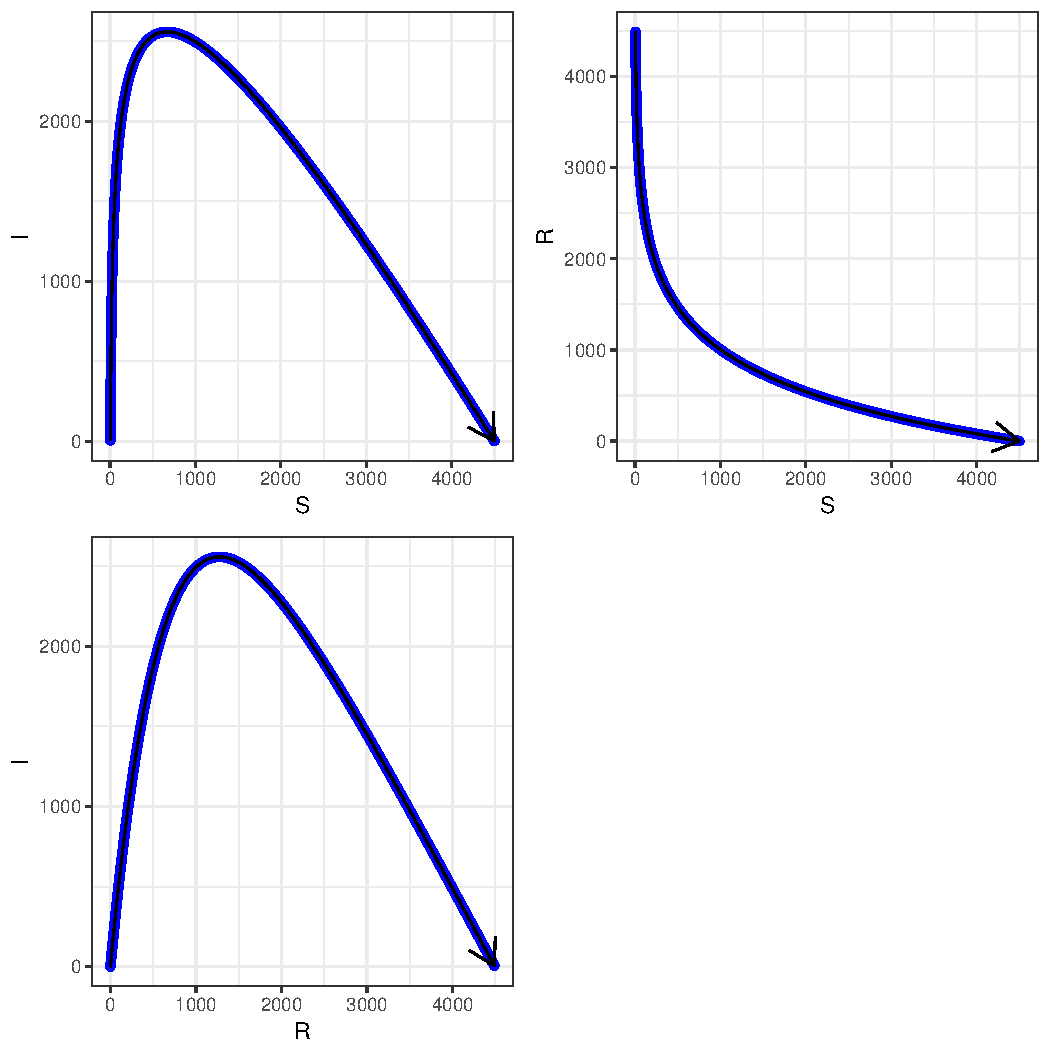
\includegraphics[width=\maxwidth]{figure/Test-1} 
\begin{kframe}\begin{alltt}
\hlstd{X}\hlopt{$}\hlstd{t} \hlkwb{<-} \hlstd{X}\hlopt{$}\hlstd{t} \hlopt{/} \hlnum{2}\hlopt{^}\hlnum{8}
\hlstd{X} \hlopt{%>%} \hlkwd{gather}\hlstd{(variable, value,} \hlopt{-}\hlstd{t)} \hlopt{%>%}
  \hlkwd{ggplot}\hlstd{(}\hlkwd{aes}\hlstd{(t, value,} \hlkwc{col}\hlstd{=variable))} \hlopt{+}
  \hlkwd{geom_point}\hlstd{()} \hlopt{+} \hlkwd{geom_line}\hlstd{()} \hlopt{+}
  \hlkwd{facet_wrap}\hlstd{(}\hlopt{~}\hlstd{variable,} \hlkwc{scales} \hlstd{=} \hlstr{'free_y'}\hlstd{,} \hlkwc{ncol} \hlstd{=} \hlnum{1}\hlstd{)}
\end{alltt}


{\ttfamily\noindent\bfseries\color{errorcolor}{\#\# Error in eval(expr, envir, enclos): could not find function "{}\%>\%"{}}}\begin{alltt}
\hlkwd{library}\hlstd{(scatterplot3d)}
\end{alltt}


{\ttfamily\noindent\color{warningcolor}{\#\# Warning: package 'scatterplot3d' was built under R version 3.3.3}}\begin{alltt}
\hlkwd{scatterplot3d}\hlstd{(X}\hlopt{$}\hlstd{S, X}\hlopt{$}\hlstd{I, X}\hlopt{$}\hlstd{R,} \hlkwc{pch} \hlstd{=} \hlnum{19}\hlstd{,}
    \hlkwc{color}\hlstd{=}\hlstr{'blue'}\hlstd{,} \hlkwc{xlab}\hlstd{=}\hlstr{'S'}\hlstd{,} \hlkwc{ylab}\hlstd{=}\hlstr{'I'}\hlstd{,} \hlkwc{zlab}\hlstd{=}\hlstr{'R'}\hlstd{)}
\end{alltt}
\end{kframe}
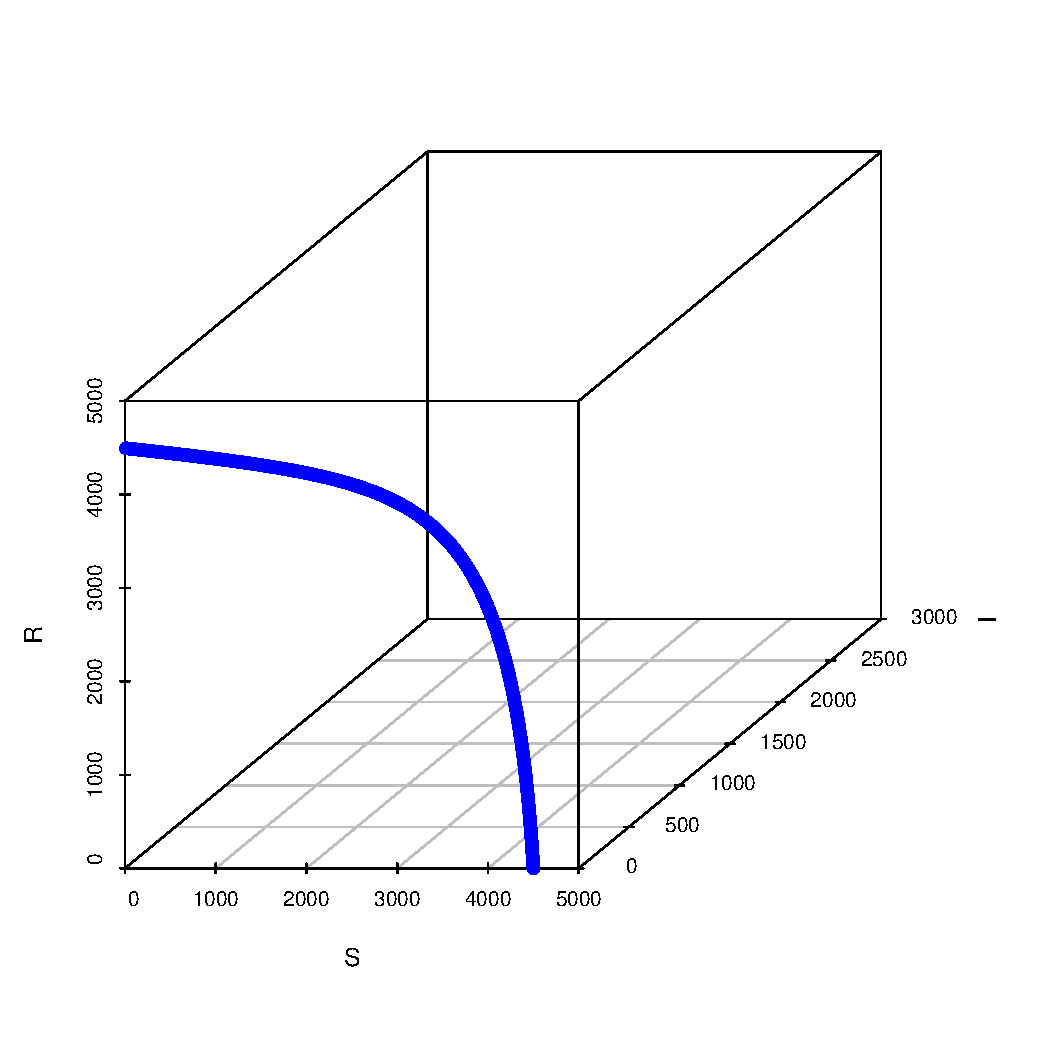
\includegraphics[width=\maxwidth]{figure/Test-2} 
\begin{kframe}\begin{alltt}
\hlstd{colfunc} \hlkwb{<-} \hlkwd{colorRampPalette}\hlstd{(}\hlkwd{c}\hlstd{(}\hlstr{"blue"}\hlstd{,} \hlstr{"red"}\hlstd{))}
\hlkwd{palette}\hlstd{(}\hlkwd{colfunc}\hlstd{(}\hlnum{1000}\hlstd{))}
\hlkwd{scatterplot3d}\hlstd{(X}\hlopt{$}\hlstd{S, X}\hlopt{$}\hlstd{I, X}\hlopt{$}\hlstd{R,} \hlkwc{pch} \hlstd{=} \hlnum{19}\hlstd{,}
    \hlkwc{color}\hlstd{=X}\hlopt{$}\hlstd{t}\hlopt{+}\hlnum{1}\hlstd{,} \hlkwc{xlab}\hlstd{=}\hlstr{'S'}\hlstd{,} \hlkwc{ylab}\hlstd{=}\hlstr{'I'}\hlstd{,} \hlkwc{zlab}\hlstd{=}\hlstr{'R'}\hlstd{)}
\end{alltt}
\end{kframe}
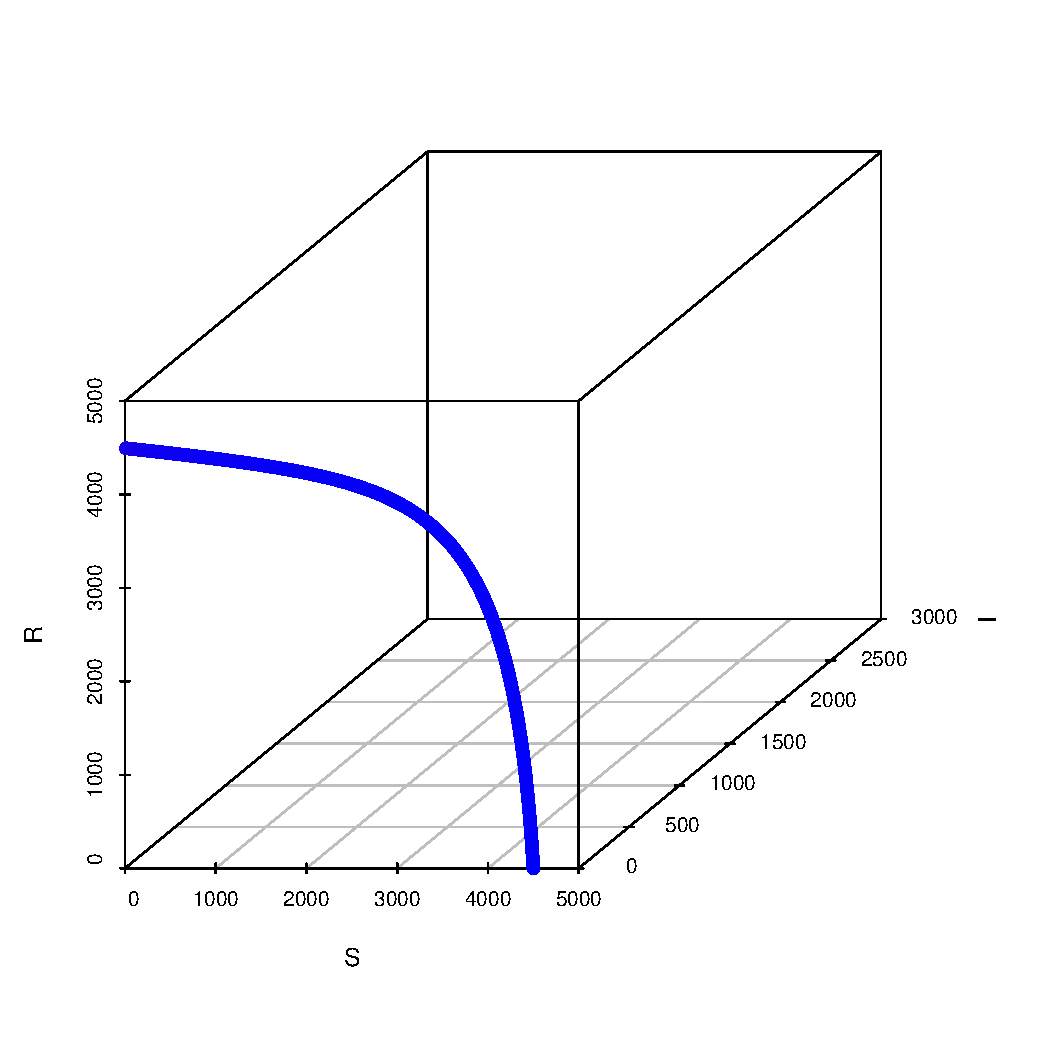
\includegraphics[width=\maxwidth]{figure/Test-3} 
\begin{kframe}\begin{alltt}
\hlcom{#Rscript -e "library(knitr); knit('ex1.Rnw')"}
\end{alltt}
\end{kframe}
\end{knitrout}

Done. 
\end{document}
